\newpage
\pagenumbering{arabic}
\section{INTRODUCTION}
Water is a fundamental requirement for all living organisms and is one of the most important resources on earth \cite{Smarzewska2021}. The rapid population growth has impacted resource utilization and led to water pollution. Wastewater consists of both liquid and solid waste generated by residential properties,
commercials and agriculture-related activities, as well as any other kind of water used by humans that is subsequently released into a sewerage system
with poor quality \cite{Prasad2020}.

Domestic wastewater can be categorized into two types, and they are greywater and blackwater. Greywater is the wastewater generated from bathtubs, laundry machines, hand basins, showers, and kitchen sinks, excluding any input from toilets. Approximately 75\% of the total household sewage is composed of greywater \cite{Eriksson2002}. Blackwater originates from toilets and contains water, urine, excrement, and toilet paper materials \cite{Paulo2013}. The composition of contaminants in wastewater may fluctuate depending on the specific industrial,
agricultural and municipal activities that discharge them. The pollutants are classified into three categories: inorganic, organic, and biological \cite{Sangeetha2023}.

The composition of the wastewater can result in adverse impacts on the environment, aquatic and wildlife populations and could potentially contaminate drinking water sources \cite{Smarzewska2021}. Organic matter can lead to oxygen depletion in rivers, lakes, and streams. Eventually, the biological decomposition of organic matter may lead to fish mortality and unpleasant smells. Also, wastewater includes nutrients that might enhance the growth of aquatic plants and may contain toxic substances that could be carcinogenic or mutagenic \cite{Prasad2020}. Therefore, wastewater treatment is essential before discharge to the water bodies.

Wastewater treatment involves separating and breaking down some of the solids that are in wastewater and turning complex organic compounds into minerals or relatively stable organic solids \cite{Sonune2004}. There are several \ac{WWTP}s that are operated under the \ac{NWSDB} in Sri Lanka, located in Moratuwa/Ratmalana, Kandy, Kurunegala, Jaela/Ekala, Seethawake, Katharagama, etc. These plants use different types of treatment processes, such as aerated lagoons, activated sludge treatment, and oxidation ditches. The activated sludge treatment process is a common technique used to treat wastewater, including municipal sewage and industrial wastewater \cite{AGUILAR2013, Chukwu2018}. Treated water from these \ac{WWTP}s' is discharged by a short sea outfall (600 m away from the seashore) and to the surface water in Sri Lanka.

\begin{sloppypar}
Sludge is identified as a solid by-product of biological wastewater treatment that contains harmful substances such as heavy metals, pathogens, and organic contaminants \cite{Wu2020}, and the wet sludge can contain up to 98\% of water content
\cite{Chan2016, SyedHassan2017}. Sewage sludge production has increased globally due to rising population, industrialization, and urbanization, and the characteristics of the sludge vary with the source of the wastewater. Dewatering and drying are important procedures to reduce the volume for easy transportation and further sludge treatment \cite{Chang2023}. 
\end{sloppypar}

With reference to the \Cref{fig:Sludge_water}, the water content can be classified as (i) free (or bulk), (ii) vicinal (or surface), (iii) interstitial, and (iv) chemically bound (or hydration) based on the interaction with sludge solid particles \cite{SyedHassan2017, Qi2020, Vaxelaire2004, Novak2006}. Free water, which can be eliminated through drainage, mechanical dewatering, or thickening, refers to water that is not connected to or affected by the suspended solid particles. It is the most readily removable water from the wet sludge. Interstitial water is confined within the fissures and interstitial spaces of the flocs and organisms.


\begin{figure}[H]
\centering
\fbox{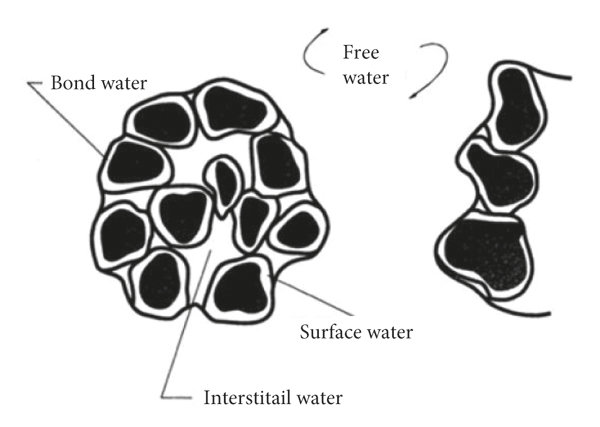
\includegraphics[width=.75\textwidth]{moisture distribution.jpg}}
\caption{Classification of water in sewage sludge}\cite{Qi2020}
\label{fig:Sludge_water}
\end{figure}

Interstitial water can be transitioned into free water when the flocs and microbial cells are eliminated. Applying mechanical energy can remove a significant amount of water by pressing it out of the sludge. Many dewatering techniques can remove both interstitial and bulk water from the sludge, and dewatered sewage sludge typically includes 73–84\% moisture \cite{Chan2016}.
 
Sewage sludge management is financially and environmentally complex due to social challenges, high treatment expenses, health risks, and limited sustainable disposal methods \cite{Fuerhacker2011}. Some disposal methods for sludge are as fertilizers, some as fuel, and some as raw materials for building materials \cite{Bratina2016}.
 
Evaluating the performance of a treatment plant involves measuring its efficiency using known indicators such as the removal of pollutants such as \ac{BOD}, \ac{COD}, and suspended solid contaminants. Operational difficulties can be detected through these evaluations and may be fixed to ensure that the plant functions properly \cite{Khan2018}. The performance efficiency of a treatment plant relies not only on its correct design and construction but also on proper operation and maintenance \cite{Kumar2010}.

 
Therefore, this study was designed to evaluate the performance of \ac{WWTP} and sludge management.


The objectives are to; 
 
 (1) evaluate the effluent quality based on the standards. 
 
 (2) analyze the removal efficiencies of the contaminants through the biological treatment.
 
 (3) analyze the sludge dewatering and drying processes.